%\documentclass[amsmath,amssymb,reprint]{revtex4-1}

%\documentclass[aps,pra,twocolumn,nopacs,superscriptaddress,groupedaddress]{revtex4}
\documentclass[aps,preprint,singlecolumn,nopacs,superscriptaddress,groupedaddress]{revtex4}

%\documentclass[twocolumn,amssymb, nobibnotes, aps, prx,nopacs,superscriptaddress, groupedaddress]{revtex4}

%\documentclass[twocolumn,amssymb, nobibnotes, aps, prx,nopacs,superscriptaddress, groupedaddress]{revtex4}


\usepackage{amsmath}
\usepackage[dvips]{graphicx}
\usepackage{epsfig}
\usepackage{tabularx}
\usepackage{color}
\usepackage[pdfpagemode=UseNone,colorlinks=true,linkcolor=blue,citecolor=blue]{hyperref}

\usepackage{soul}
\usepackage{gensymb}

%\usepackage{setspace}

%\usepackage{subcaption}
%\usepackage{float}


\newcommand{\blue}[1]{{\color[rgb]{0,0,1}#1}}
\newcommand{\red}[1]{{\color[rgb]{1,0,0}#1}}
\newcommand{\green}[1]{{\color[rgb]{0,0.7,0}#1}}

\newcommand{\redd}[1]{{\color[rgb]{0.7,0,0}#1}}

\renewcommand\Re{\operatorname{Re}}
\renewcommand\Im{\operatorname{Im}}
\newcommand{\fixme}[1]{\textcolor{red}{#1}}

\newcommand{\di}{i}  




\begin{document}



\title[]{Strong coupling and dark modes in the motion of a pair of levitated nanoparticles }


\author{A. Pontin}
\email{antonio.pontin@cnr.it}
\affiliation{CNR-INO, largo Enrico Fermi 6, I-50125 Firenze, Italy}

\author{Q. Deplano}%
\affiliation{Dipartimento di Fisica e Astronomia, Università degli Studi di Firenze, via Sansone 1, I-50019 Sesto Fiorentino, Italy}%
\affiliation{INFN, Sezione di Firenze, via Sansone 1, I-50019 Sesto Fiorentino, Italy}

\author{A. Ranfagni}%
\affiliation{Dipartimento di Fisica e Astronomia, Università degli Studi di Firenze, via Sansone 1, I-50019 Sesto Fiorentino, Italy}%

\author{F. Marino}%
\affiliation{CNR-INO, largo Enrico Fermi 6, I-50125 Firenze, Italy}
\affiliation{INFN, Sezione di Firenze, via Sansone 1, I-50019 Sesto Fiorentino, Italy}


\author{F. Marin}
\email{marin@fi.infn.it}
\affiliation{CNR-INO, largo Enrico Fermi 6, I-50125 Firenze, Italy}
\affiliation{Dipartimento di Fisica e Astronomia, Università degli Studi di Firenze, via Sansone 1, I-50019 Sesto Fiorentino, Italy}%
\affiliation{INFN, Sezione di Firenze, via Sansone 1, I-50019 Sesto Fiorentino, Italy}
\affiliation{European Laboratory for Non-Linear Spectroscopy (LENS), Via Carrara 1, I-50019 Sesto Fiorentino, Italy}


\begin{abstract}
We experimentally investigate a system composed of two levitating nanospheres whose motions are indirectly coupled via coherent scattering in a single optical cavity mode. The nanospheres are loaded into a double longitudinal tweezer created with two lasers at different wavelengths, where chromatic aberration leads to the
formation of two separate trapping sites. We achieve strong coupling between each pair of modes in the transverse plane of the tweezer, as demonstrated by the avoided crossings observed when tuning the eigenfrequencies of the motion of one nanosphere by varying its optical potential depth. Remarkably, we show the emergence of dark modes in the overall coupled motion. The dynamics can be described in terms of spin-1/2 matrices, and the observed features are ubiquitous in a variety of classical and quantum systems. As such, our experiment will allow us to explore the classical analog of typically quantum dynamics, and in further developments to investigate the transition to the quantum domain by lowering the decoherence rate and creating stationary entanglement, as well as implementing non-stationary protocols.
\end{abstract}

\maketitle
Levitated optomechanical systems have shown a fast development over the last decade, and they are a promising platform for the exploration of quantum mechanics in the mesoscopic mass range~\cite{Millen2020Optomechanics,Bassi2013Models}.  Nowadays, the motional ground state for the center of mass of an optically levitated nanoparticle can be routinely prepared, both in free space by feedback ~\cite{Magrini2021,novotny2021_GS,Kamba2022Optical} and through cavity-assisted cooling~\cite{Delic2020science,Ranfagni2021Two-dimensional,Piotrowski2023Simultaneous,Deplano2024Highpurity}. Levitated objects are also seen as attractive sensors both for fundamental science topics, such as dark matter searches~\cite{Monteiro2020Search,Moore2021Searching, Kilian2024Darkmatter} or gravitational wave detection~\cite{Arvanitaki2013Detecting,Aggarwal2022Searching}, and for technological applications~\cite{Monteiro2017Optical,Rademacher2019Quantum,Ahrens2024Levitated}. An additional feature of levitation, compared to clamped optomechanical systems, is the possibility of accessing and manipulating the rotational degrees of freedom, which offer unique opportunities~\cite{Muddassar2018Precession,tongcangli_5D,novotny_libration_fbk2021,Pontin2023Simultaneous,Zielinska2023Controlling}. 

In recent years, an emerging topic within the field has been the study of multiparticle interactions.  Indeed, coupling between two particles has been explored on different platforms including electrodynamic and gravito-optical traps, and optical tweezers. These experiments have demonstrated sympathetic cooling~\cite{Arita2022Alloptical,Lika2023Colddamping, penny2023Sympathetic, Bykov2023_3Dsympathetic} and squeezing~\cite{penny2023Sympathetic}, cold damping~\cite{Vijayan2022Scalable}, optical binding yielding anti-reciprocal coupling~\cite{Rieser2022Tunable} and strong Coulomb coupling~\cite{Deplano2024Coulomb}. This body of work represents the first building block toward more enticing experiments  such as the generation and observation of entanglement between mesoscopic objects~\cite{Chauhan2020Stationary,Brando2021Coherent,Winkler2024Steady-state}, and the exploration of the quantum nature of gravity~\cite{Bose2017spin}.

A recent work ~\cite{Vijayan2024Cavity-mediated} showed strong coupling between pairs of collinear oscillation modes of two levitated nanoparticles. The long range interaction was mediated by an optical cavity in the Doppler regime, exploiting coherent scattering (CS)~\cite{Vuletic2000Laser,novotny_CS_2019,Delic_CS_2019,toros2020Quantum,toros2021Coherent}.
Here, we introduce a different approach, where the two particles are loaded in a bichromatic longitudinal tweezer~\cite{Deplano2024Coulomb}  and the CS interaction operates in the resolved sideband regime. 
This method allows to vary the optical potential independently of the CS coupling term. Furthermore, strong coupling between all modes in the tweezers transverse plane is achieved, as demonstrated by the observed avoided crossings that, for each mode pair, display frequency splittings of $\approx 1$ kHz, significantly exceeding the modes linewidths.

More importantly, we show the emergence of a dark mode in the upper branch of the crossing. 
When considering the motion in a tweezer polarization plane, say $x$ and $y$ modes, it has been previously noted that a single particle interacting by CS with a cavity mode can be described in terms of spin 1 matrices~\cite{toros2021Coherent}, which are usually associated with purely quantum systems. For sufficiently strong coupling, this leads to a three-mode avoided crossing at the tripartite resonance with a dark mode at the center of the crossing~\cite{Ranfagni2021Vectorial}. The same description can be used when considering two modes belonging to different particles.

In the present experiment, we are exploring the weak coupling limit for the interaction of each individual particle with the cavity. This allows to trace out the cavity and describe the dynamics as that of two strongly coupled motional modes \cite{Vijayan2024Cavity-mediated}. Thus, the dynamics can be described in terms of spin 1/2 matrices with an obvious parallel to a quantum two-level system. Indeed, the same features presented here in the classical regime can be found in disparate quantum systems. A first example is a pair of single molecules directly coupled by a dipole-dipole interaction~\cite{Trebbia2022Tailoring}, in which case the bright/dark mode is typically discussed in terms of sub/superradiance. A second example is provided by two transmons qubits coupled by a superconducting cavity, where the bright/dark mode represents the antisymmetric/symmetric superposition of the two qubit states~\cite{Majer2007Couplingsuperconducting}. Other notable examples can be found in Refs.~\cite{Evans2018Photon-mediated,Filipp2011Multimode,Leseleuc2017Optical}.

\begin{figure}%[ht]
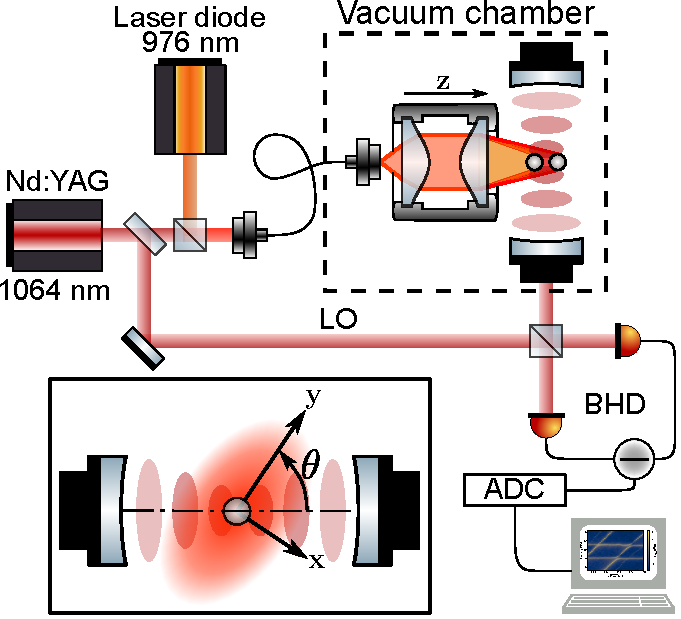
\includegraphics[width=8.6cm]{fig1_v2.pdf}
\caption{Overview of the experiment. A bi-chromatic optical tweezer allows to confine nanoparticles in two trapping sites separated by $r_{12}=9\pm1\,\mu$m. The two particles are placed at the center of a high finesse optical cavity implementing a coherent scattering approach. The particles motion is measured through a balanced heterodyne detection (BHD). The tweezer polarization is set at an angle $\theta\approx45$°, giving similar optomechanical couplings for the $x$ and $y$ directions. LO: local oscillator, ADC: analog-to-digital converter.  
}\label{fig1}
\end{figure}

\emph{Experimental setup} - We implement a fiber-based approach to obtain our optical tweezer. Light from a polarization maintaining (PM) fiber is first collimated by an aspheric lens (focal length $f=18.4$\,mm) and subsequently refocused by a second asphere ($f=3.1$\,mm). This generates a sub-$\mu$m waist. Silica particles are initially loaded in an auxiliary tweezer housed in a loading chamber, and then transferred to the main tweezer~\cite{Calamai2021Transfer}. The main aspheric doublet is mounted on a 3 axes translational stage which allows nanometric positioning at the center of an optical cavity.  

We inject light into the PM fiber from two sources, a Nd:YAG at $1064$\,nm  and a diode laser at $976$\,nm, which are overlapped at the fiber input with orthogonal polarizations. Chromatic aberration of the doublet guaranties that the foci occur at different positions along the tweezer field propagation direction ($z$ axis). For our wavelengths, the separation between the two spots is estimated to be $r_{12}=9\pm1\,\mu$m. 

The optical cavity has a quasi-concentric configuration with identical concave mirrors, a free spectral range FSR$=3.07$\,GHz and a waist of $31\,\mu$m. The cavity full linewidth is $\kappa/2\pi=57$\,kHz at $1064$\,nm while the cavity mirrors are effectively transparent at $976$\,nm. A second Nd:YAG locked to the optical cavity provides a reference to offset phase-lock the $1064$\,nm tweezer light. The frequency offset is set at a frequency of FSR$+\Delta/2\pi$ allowing precise control of the tweezer field detuning $\Delta$ with respect to the cavity resonance.

\emph{Model} - Both particles couple to the cavity mode through a CS interaction ~\cite{Vuletic2000Laser,novotny_CS_2019,Delic_CS_2019,toros2020Quantum,toros2021Coherent}. Light directly scattered by the particles is injected into the cavity mode giving rise to a coupling between the intracavity field and the particles motion.  Contrary to the typical scenario~\cite{Vijayan2024Cavity-mediated}, the light generating the second trap, at $976$\,nm, does not participate in the coherent scattering interaction. However, the particle in this trap still scatters $1064$\,nm light into the cavity albeit with reduced power. We can write the electric field of the $1064$\,nm light at particle 2 as $E_2=\zeta\,E_1\,e^{i\varphi}$. Here, $E_1$ is the field at the $1064$ focus while $\zeta$ and $\varphi$ account for the different amplitude and phase at the $976$ focus.  These two parameters fully characterize the relative strength of the CS interaction for the second particle. Based on a Gaussian approximation of the field propagation we can estimate $\zeta=0.28\pm0.03$. Notice that $\zeta<1$ due to the geometry of the system.


The experimental results presented here explore only the weak coupling limit of the interaction between motion and cavity field. In this regime, modeling of the experiment simplifies considerably, since the cavity can be traced out. It can be shown \cite{Vijayan2024Cavity-mediated,supp} that the cavity mediated coupling between the two particles assumes the following form 

\begin{equation}\label{eq_2} 
   G_{\alpha\beta}=\frac{g_\alpha g^*_{\beta}}{\Delta - \omega_\beta - \mathrm{i} \kappa/2} + \frac{g^*_\alpha g_{\beta}}{\Delta + \omega_\beta +\mathrm{i} \kappa/2}
\end{equation}

\noindent where $g_i$ is the coupling rate between motional mode \emph{i} and cavity field, and $\omega_i$ is the modal eigenfrequency. Eq.~(\ref{eq_2}) allows to focus directly on the motional dynamics of the two particles. In general, $G_{\alpha\beta}\neq G_{\beta\alpha}$ so that the interaction can be non-reciprocal. Maximal non-reciprocity occurs at a phase $\varphi=\pi/2$, whereas a purely conservative interaction is recovered for $\varphi=0$.   

\begin{figure}%[ht]
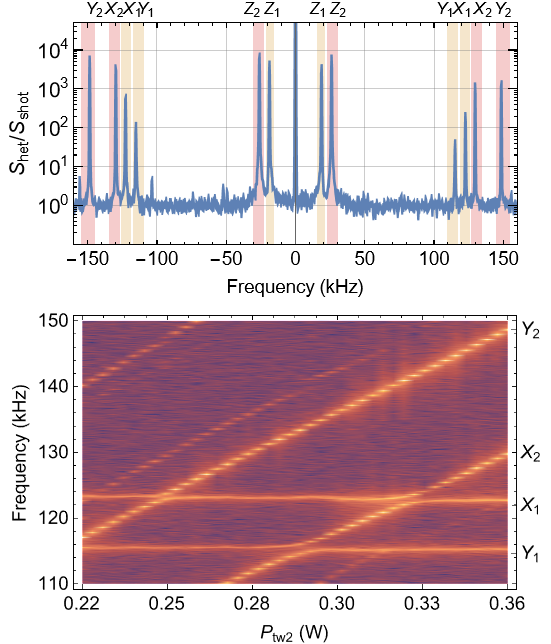
\includegraphics[width=8.6cm]{fig2_tmp_scan_b.png}
\caption{Experimental spectra. a) Heterodyne spectrum of the cavity output normalized to the shot noise. The spectral peaks of the two particles degrees of freedom $(z_1,x_1,y_1,z_2,x_2,y_2)$ are identified with yellow and red shaded regions for particle 1 and 2, respectively. b) Spectrogram of the heterodyne power spectral density (PSD) as a function of the trapping power $P_{\text{tw2}}$ of the $976$\,nm field. The power is varied in discrete steps. Three avoided crossings are clearly visible at $P_{\text{tw2}}=(0.32,0.29,0.24)$\,W. This demonstrates an effective direct coupling between mechanical modes belonging to different particles.
}\label{fig2}
\end{figure}


\emph{Experiment} - We trap two silica particles of nominal diameter $125$\,nm. The power of the $1064$\,nm field is kept constant throughout the experiment at $P_{\mathrm{tw1}}=250$\,mW. This gives trap frequencies of $(\omega_{z1},\omega_{y1},\omega_{x1})/2\pi=(19,117,124)$\,kHz for the first particle. The power of the $976$\,nm light can be varied  from $P_{\mathrm{tw2}}=360$\,mW down to $220$\,mW. The lower bound is set to avoid particle loss. At the highest power, we have $(\omega_{z2},\omega_{y2},\omega_{x2})/2\pi=(28,148,129)$\,kHz, and the frequency difference ensures that  the two particles can be considered as independent. The $1064$\,nm field polarization is linear and set at $\theta\simeq45\degree$, where $\theta$ is the angle between the $y$ direction and the cavity axis, so that we expect $g_{x_i}\simeq g_{y_i}$. We show in Fig.~\ref{fig2}\,a a heterodyne spectrum taken at a pressure of $5\times10^{-6}$\,mbar with a red detuning set at $\Delta/2\pi=-425$\,kHz. All spectral peaks of the two particles degrees of freedom are clearly recognizable. The two particles are charged with measured charges of $ |q_1|= (89\pm10)\,q_e$ and $|q_2|= (71\pm10)\,q_e$ where $q_e$ is the elementary charge~\cite{Deplano2024Coulomb}. 

The two particles are positioned close to the cavity axis, and the position along the cavity standing wave is set by minimizing the total light scattered into the cavity mode. This does not necessarily occur at a cavity node as is typical in single particle experiments~\cite{supp}.

By controlling the power of the $976$\,nm field we can tune its trap frequencies to be resonant to those of the $1064$\,nm. Since the foci parameters are sufficiently different, the resonance condition is achieved only for a single pair of modes at a time. We show in Fig.~\ref{fig2}\,b) a spectrogram obtained by scanning $P_{tw2}$, displaying  the frequency region around the resonances of the modes in the tweezers transverse plane (i.e., $x_i,y_i$). The power is changed in discrete steps of $3.5$\,mW. Three avoided crossings are clearly observable, and a fourth remains just outside the scanning range. Fitting with Lorentzian shapes the four spectral peaks at each step, we reconstruct the behavior of the four eigenfrequencies of the system. 


\begin{figure}[ht]
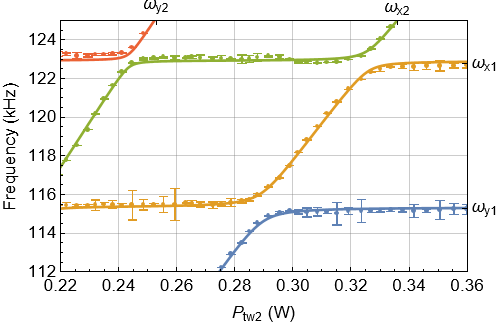
\includegraphics[width=8.6cm]{fig3_tmp_fit_eigenvalues.png}
\caption{Measurement of the system eigenfrequencies for the motion in the tweezers transverse plane. The experimental data (markers with error bar) are shown along with the modeled eigenfrequencies (solid lines). Three avoided crossings are visible, allowing to infer effective direct coupling rates of $(g_{x1,x2}, g_{y1,x2}, g_{x1,y2})/2\pi=(0.61, 0.6, 0.51)$\,kHz respectively.
}\label{fig3}
\end{figure}

We model the experiment considering nominal particle and cavity parameters, in line with previous experiments~\cite{Ranfagni2021Two-dimensional}, and fit the measured frequency splittings to extract the cavity drive ratio $\zeta$, relative field phase $\varphi$ and the initial position in the cavity standing wave~\cite{supp}. The resulting eigenfrequencies are shown in Fig.~\ref{fig3} together with the experimental data, demonstrating excellent agreement.

The fitting procedure returns a phase $\varphi=(172\pm 3) \degree$, thus very close to optimal for a purely conservative interaction, and a coupling strength $\zeta=0.35 \pm 0.015$ which is in fairly good agreement with the crude estimate using a Gaussian approximation.  For the particle in the $1064$\,nm trap we find $(g_{x1}, g_{y1})/2\pi=(18.1\pm 0.6, 17.3\pm 0.5)$\,kHz, while for the second particle we have $(|g_{x2}|, |g_{y2}|)/2\pi=(P_{0}/P_{tw2})^{1/4} (7.0\pm 0.3, 6.0\pm 0.2)$\,kHz where $P_{0}=220$\,mW is a reference power.
 


\emph{Discussion} - The cavity mediated interaction between the two particles can be described as an effective direct coupling $g_{\alpha,\beta}=\mid G_{\alpha,\beta} \mid_{\omega_{\alpha}=\omega_{\beta}}$. The normal mode splitting at the avoided crossings is then given by $\delta_{\alpha,\beta}=2 g_{\alpha,\beta}$. For the three visible crossings, occurring at a power of $P_{\mathrm{tw2}}=(326,291,243)$\,mW, we find $(\delta_{x1,x2}, \delta_{y1,x2}, \delta_{x1,y2})/2\pi=(1.22\pm 0.06, 1.20\pm 0.06, 1.02\pm 0.06)$\,kHz respectively. The fourth splitting, occurring at $P_{\mathrm{tw2}}=214$\,mW, can be estimated to be $\delta_{y1,y2}/2\pi=0.78\pm 0.05$\,kHz.

In the case of interacting modes of different linewidths \green{$\gamma_i$}, we can define the strong coupling threshold as $g_{\alpha,\beta} > (\gamma_\alpha +\gamma_\beta)/4$. The largest measured linewidth, dominated by the optomechanical interaction, is  $\gamma_{\text{opt}}/2\pi =109\pm 20$ \,Hz. Taking this as upper-bound ensures that all crossings are well within the strong coupling regime. 

\begin{figure}[t]
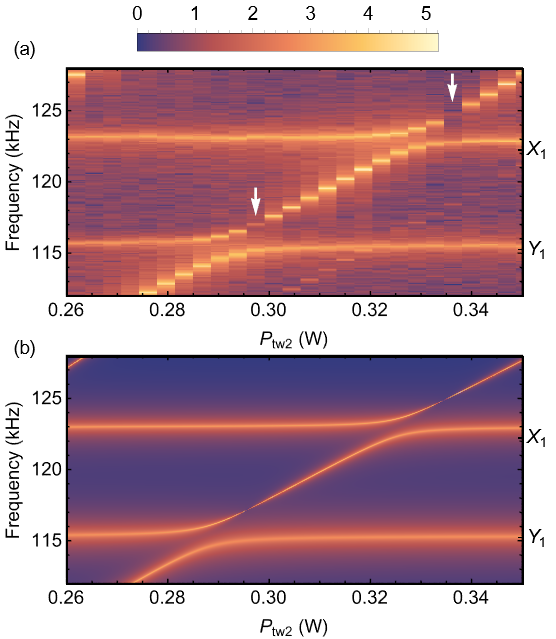
\includegraphics[width=8.6cm]{fig4_tmp_dark_v3.png}
\caption{Dark mode formation. a) Spectrogram of the Heterodyne PSD as a function of the trapping power $P_{\text{tw2}}$ of the $976$\,nm field around the avoided crossings at $P_{\text{tw2}}=(323,289)$\,mW which shows the formation of dark modes, marked with arrows, on the upper branches. b) analytical heterodyne spectrogram calculated with fitted parameters with the only exception of setting the phase $\varphi=\pi$ to highlight the dark mode.
}\label{fig4}
\end{figure}

To understand the formation of the dark mode at an avoided crossing, let us first consider the simplified scenario of two motional modes of frequencies $\omega_1=\omega_0-\delta \omega$ and $\omega_2=\omega_0+\delta \omega$ with identical coupling rates to the cavity $g=g_1=g_2$, which implies $\varphi=0$. In the large detuning limit, i.e. $|\Delta|\gg \kappa, \omega_j$, the eigenvalues of the dynamical matrix~\cite{supp} at the crossing ($\delta\omega=0$) are given by $(\lambda_+,\lambda_-)=(\omega_0,\,\omega_0+4g^2/\Delta+\di\,4\kappa g^2 \omega_0/\Delta^3)$. It is clear that one mode is down-shifted and broadened (lower branch $\lambda_-$) while the other is completely unaffected by the cavity (upper branch $\lambda_+$) and can then be identified as the dark mode. However, when a gain imbalance is present, the real and imaginary parts of the eigenvalues are affected differently. If we now consider $g_2=\zeta\,g$, the minimal distance between the pair of eigenfrequencies, defining the position of the avoided crossing, occurs at $\delta\omega=(1-\zeta^2)g^2/\Delta$ where $\mathrm{Re}[\lambda_{\pm}]=\omega_0+(\zeta\mp1)^2 g^2/\Delta$, but it is still at $\delta\omega=0$ that the imaginary part of $\lambda_+$ vanishes, and $\mathrm{Im}[(\lambda_+,\lambda_-)]=(0,\,(1+\zeta^2)\,2\kappa g^2 \omega_0/\Delta^3)$. In other words, the dark mode always forms at the crossing of the bare frequencies, not at the position of minimal distance between optically-shifted effective frequencies.

In fact, this is the scenario that can be observed in the experimental spectrogram of Fig.~\ref{fig4}~a). For both avoided crossings shown, the amplitude of the upper branch significantly dims at a power corresponding to a $\delta\omega$ higher than that of the crossing, as expected. The amplitude does not completely vanish for three reasons: \emph{i}) the dark mode only appears for $\varphi=0$, away from this value one should rather consider a "pseudo"-dark mode, with a contrast quickly vanishing as the phase moves away from the optimal value. \emph{ii}) The region over which the dark mode manifests itself is narrow compared to the resolution of the power scan. \emph{iii}) Due to the Coulomb force between the charged particles, changing the trap potential results in a shift of the equilibrium position, i.e., the particles separation, of the order of few $100$\,nm. This introduces a power dependence on the relative phase of the fields $\varphi$, though with negligible effect on $\zeta$. For comparison, we show in Fig.~\ref{fig4}\,b) the analytical heterodyne spectrogram. This is calculated with the fitted parameters except for the phase $\varphi$ and the effect of the Coulomb shift, which have been both set to zero to show the maximum contrast of the dark mode. 

As mentioned in the previous paragraph, the Coulomb force is not negligible, due to its effect on the position-dependent field phase. Coulomb coupling affects the dynamics of the mode pairs $(x_1,x_2)$ and $(y_1,y_2)$ with a coupling rate estimated to be $g_C/2\pi\simeq120$\,Hz, and it thus introduces a minor contribution to the corresponding avoided crossings. To model the eigenfrequencies shown in Fig.~\ref{fig3}, both the direct effective couplings and the Coulomb force are fully included in the model. More details can be found in~\cite{supp}.  On the other hand, at the separation $r_{12}=9\,\mu$m optical binding can be neglected.


In conclusion, we exploited a novel scheme to confine two nanoparticles in separated trapping sites of a double optical tweezer, and place them at the center of a high finesse optical cavity. This allowed us to exploit a coherent scattering interaction to generate an effective direct coupling between interparticle modes, mediated by the cavity. We have directly shown the appearance of three avoided crossings between pairs of motional modes in the tweezer polarization plane with splittings of $\approx1$\,kHz. A fourth remains just outside our scanning range, but is predicted to be of the same order. All crossings are well within the strong coupling regime. We have also shown that the effective direct coupling leads to the formation of a dark mode in the upper branch of the avoided crossing spectrogram, which occurs when the bare frequencies are degenerate.

These features are quite common across a variety of physical systems, including those operating deeply in the quantum regime~\cite{Trebbia2022Tailoring,Majer2007Couplingsuperconducting}. Indeed, an experiment in the classical regime can represent the classical analog of quantum dynamical phenomena including, for example, Rabi oscillations and Ramsey fringes~\cite{Ivakhnenko2018Simulating,Frimmer2014TheclassicalBloch}, which could be explored with our system. Of course, an even more interesting scenario would be achieved by preparing the two particles in their mechanical ground state to pursue the generation of stationary Gaussian entanglement \cite{Chauhan2020Stationary}, as well as non-stationary quantum protocols \cite{Rudolph2020,Brando2021Coherent}. To achieve this, some upgrades for the current setup will be necessary. However, these are fully achievable with the technology currently available. For example, a widely tunable light source for the second tweezer will allow control of the interaction phase $\varphi$ and particles separation $r_{12}$, which directly affects the interaction strength $\zeta$. It is also possible to envision a regime where both cavity-mediated interaction and optical binding are relevant. Lastly, a doubly resonant cavity at both $1064$\,nm and $976$\,nm, would represent a novel approach within the CS framework with a much larger parameter space available to tailor the interaction.

We acknowledge financial support from PNRR MUR Project No. PE0000023-NQSTI and by the
European Commission-EU under the Infrastructure I-PHOQS “Integrated Infrastructure Initiative
in Photonic and Quantum Sciences ” [IR0000016, ID D2B8D520, CUP D2B8D520].



\bibliographystyle{nicebib}
\bibliography{main_bib}



\end{document} 

